\documentclass[a4paper,12pt]{scrartcl}
\usepackage{a4wide}
\usepackage[left=2cm, right=2cm, top=3cm]{geometry}
\usepackage{graphics}
\usepackage{mathtools}
\usepackage{amsmath, amssymb} 
\usepackage[utf8]{inputenc}
\usepackage[ngerman]{babel}
\usepackage{hyperref}
\usepackage{enumitem}
\usepackage{booktabs}
\usepackage{aligned-overset}  % Um bei Align die Gleichheitszeichen übereinander zu haben
\usepackage[version=4]{mhchem}
\usepackage{cancel}
\usepackage{wrapfig}
\usepackage{marvosym}
\usepackage[headsepline]{scrlayer-scrpage}
\usepackage{subcaption}
\usepackage{tabularx}
\usepackage{environ}
\usepackage{natbib}
\usepackage{tikzsymbols}
\usepackage[skins, xparse, breakable]{tcolorbox}
\usepackage{xcolor}
\usepackage{dsfont}
\usepackage{pdfpages} % https://www.namsu.de/Extra/pakete/Pdfpages.html
\allowdisplaybreaks  % Damit Align-Umgebungen umgebrochen werden können



% Set to 1 (only selection) or 0 (full script)
\newcounter{reduce_to_selection}
\setcounter{reduce_to_selection}{0}
% \setcounter{reduce_to_selection}{1}
% \includeonly{Woche07}


\newcommand{\Tipps}[2]{
    \ifnum\value{reduce_to_selection}=1 {
        \subsection{Tipps zu den Aufgaben von Blatt #1}
        \Disclaimer{}\\
        #2
    }
    \fi
}



\bibpunct{[}{]}{;}{a}{}{,}
\usepackage{scalerel}
\def\stretchint#1{\vcenter{\hbox{\stretchto[440]{\displaystyle\int}{#1}}}}
\def\bs{\mkern-12mu}
\pagestyle{scrheadings}
\clearpairofpagestyles


\numberwithin{equation}{section}
\let\oldsection\section  % Footnotecounter resetten
\renewcommand{\section}{\setcounter{footnote}{0}\oldsection}
\renewcommand{\thefootnote}{\Roman{footnote}}
\setlist[itemize]{topsep=1pt, itemsep=0pt, parsep=0.5pt}  % Itemize manipulieren
\setlist[enumerate]{topsep=1pt, itemsep=0pt, parsep=0.5pt}  % Itemize manipulieren


%%%%%%%%%%%%%%%%%%%%%%%%%%%%% Neue Umgebungen
\NewEnviron{Answer}
{%
\noindent
\rotatebox[origin=c]{180}{%
\noindent
\begin{minipage}[t]{\linewidth}
\BODY
\end{minipage}%
}%
}%

\newcommand{\C} {\mathbb{C}} 
\newcommand{\N} {\mathbb{N}} 
\newcommand{\Q} {\mathbb{Q}} 
\newcommand{\R} {\mathbb{R}}
\newcommand{\Z} {\mathbb{Z}}

\definecolor{mygreen}{RGB}{17,100,8}
\newtcolorbox[auto counter,number within=section]{Def}[2][]{%
breakable, enhanced, sharp corners, rounded corners=northwest, rounded corners=southeast, colback=blue!5!white,colframe=black!75!black,fonttitle=\bfseries,
title=Definition~\thetcbcounter: #2,#1}

\newtcolorbox[auto counter, number within=section]{Satz}[3][]{%
breakable, enhanced, sharp corners, rounded corners=southwest, rounded corners=northeast, colback=blue!5!white,colframe=red!75!black,fonttitle=\bfseries,
title=#2~\thetcbcounter: #3,#1}

\newtcolorbox[auto counter,number within=section]{Beispiel}[2][]{%
breakable, enhanced, colback=blue!5!white,colframe=blue!75!black, fonttitle=\bfseries,
title=Beispiel~\thetcbcounter: #2,#1}

\newtcolorbox[auto counter,number within=section]{Wiederholung}[2][]{%
breakable, enhanced, sharp corners, colback=green!5!white,colframe=mygreen!75!black, fonttitle=\bfseries,
title=Wiederholung~\thetcbcounter: #2,#1}

\makeatletter
\def\iddots{\mathinner{\mkern1mu\raise\p@
\vbox{\kern7\p@\hbox{.}}\mkern2mu
\raise4\p@\hbox{.}\mkern2mu\raise7\p@\hbox{.}\mkern1mu}}
\makeatother


\makeatletter
\newcommand{\tx}[1]{\text{#1}}
\newcommand{\Menge}[2]{\left\{#1\furdas#2\right\}}
\newcommand{\MengeDirekt}[1]{\left\{#1\right\}}
\newcommand{\diff}[2]{\frac{\text{d}#1}{\text{d}#2}}
\newcommand{\diffp}[2]{\frac{\partial#1}{\partial#2}}
\newcommand{\BiFo}[1]{\left\langle#1\right\rangle}
\newcommand{\Norm}[1]{\left|\left|#1\right|\right|}
\newcommand{\BiFoLeer}{\left\langle\cdot,\cdot\right\rangle}
\newcommand{\NormLeer}{\left|\left|\cdot\right|\right|}
\newcommand{\Spoiler}[1]{Hier werden wir nach Abgabe des Blattes den Lösungsweg skizzieren.}
\newcommand{\Matrix}[1]{\begin{pmatrix}#1\end{pmatrix}}
\newcommand{\MatrixAbs}[1]{\begin{vmatrix}#1\end{vmatrix}}
\newcommand{\MatrixInline}[1]{\left(\begin{smallmatrix}#1\end{smallmatrix}\right)}
\newcommand{\MatrixInvertieren}[2]{\left(\begin{matrix}#1\end{matrix}\,\left|\,\begin{matrix}#2\end{matrix}\right.\right)}
\newcommand{\Span}[2]{\text{span}\left\{#1\furdas#2\right\}}
\newcommand{\Spann}[1]{\text{span}\left\{#1\right\}}
\newcommand{\EinheitsN}{\mathds{1}_n}
\newcommand{\red}[1]{\textcolor{red}{\textbf{#1}}}
\newcommand{\blue}[1]{\textcolor{blue}{#1}}
\newcommand{\UausC}{Sei $U\subset\mathbb{C}$ offen}
\newcommand{\Res}{\text{Res}}
\newcommand{\qedsquare}{\hfill $\square$}
\newcommand{\qed}{\hfill \textbf{q.e.d.}}
\newcommand{\furdas}{\,|\,}
\newcommand{\mybox}[1]{\parbox[t]{8.5cm}{#1}}
\newcommand{\myboxU}[1]{\parbox[b]{8.5cm}{#1}}
\newcommand{\Zz}[1]{\textbf{Beh.}: \textbf{\textit{#1}}\\}
\newcommand{\Zb}[1]{\textbf{Bew.}: \blue{#1}\qedsquare}
\newcommand{\ZbOhne}[1]{\textbf{Bew.}: \blue{#1}}
\newcommand{\Skript}{\href{https://www.math.uni-hamburg.de/home/lentner/MfPh1/SkriptMfP1Lentner2020.pdf}{Skript}}
\newcommand{\Limes}[1]{\lim_{#1\rightarrow\infty}}
\newcommand{\LimesSum}[1]{\sum_{#1=0}^\infty}
\newcommand{\LimesSumOne}[1]{\sum_{#1=1}^\infty}
\newcommand{\LimesXiToX}{\lim_{\xi\to x}}
\newcommand{\SinusReihe}{\LimesSum{k}(-1)^k\frac{z^{2k+1}}{(2k+1)!}}
\newcommand{\KosinusReihe}{\LimesSum{k}(-1)^k\frac{z^{2k}}{(2k)!}}
\newcommand{\ExpReihe}[1]{\LimesSum{k}\frac{#1^{k}}{k!}}
\newcommand{\Cases}[1]{\begin{cases}#1\end{cases}}
\newcommand{\Id}{\text{Id}}
\newcommand{\BracedIn}[1]{\left({#1}\right)}
\newcommand{\BracedInSqr}[1]{\left[{#1}\right]}
\newcommand{\Abs}[1]{\left|{#1}\right|}
\newcommand{\artanh}{\text{artanh}}
\newcommand{\arsinh}{\text{arsinh}}
\newcommand{\arcosh}{\text{arcosh}}
\newcommand{\Disclaimer}{\textcolor{blue}{
$\left[\,\text{\parbox{0.95\textwidth}{\vspace{0.1cm}\textit{\textbf{Hinweis:}\\
Da wir euch offiziell nichts vorsagen sollen (was ja auch sinnvoll ist), sind die Tipps sehr allgemein gehalten. Hoffentlich helfen sie euch trotzdem, Ansätze zu finden, falls ihr mal nicht weiter kommt.\\
Bei konkreten Fragen helfen wir gerne persönlich.\vspace{0.1cm}}}}\,\right]$
}}
\newcommand{\Einleitung}[1]{\subsection*{Ausblick}
    \textcolor{blue}{\textit{#1}}}
\newcommand{\IV}{\text{IV}}
\newcommand{\im}{\text{im}}
\newcommand{\Abb}{\text{Abb}}
\newcommand{\Bij}{\text{Bij}}
\newcommand{\I}{\text{I}}
\newcommand{\II}{\text{II}}
\newcommand{\III}{\text{III}}
\newcommand{\card}{\text{card}}
\newcommand{\diag}{\text{diag}}
\newcommand{\grad}{\text{grad}}
\newcommand{\Hess}{\text{Hess}}
\newcommand{\rot}{\text{rot}}
\newcommand{\divv}{\text{div}}
\newcommand{\Diff}{\text{Diff}}
\newcommand{\Met}{\text{Mat}}
\newcommand{\Tr}{\text{Tr}}
\newcommand{\rg}{\text{rg}}
\newcommand{\End}{\text{End}}
\newcommand{\Aut}{\text{Aut}}
\newcommand{\GL}{\text{GL}}
\newcommand{\SL}{\text{SL}}
\newcommand{\ad}{\text{ad}}
\newcommand{\sgn}{\text{sgn}}
\makeatother
%%%%%%%%%%%%%%%%%%%%%%%%%%%%%%
\let\oldhref\href
\renewcommand{\href}[2]{\oldhref{#1}{\underline{\bfseries#2}}}
\renewcommand{\Re}{\text{Re}}
\renewcommand{\Im}{\text{Im}}
\newcommand{\rvec}{{\Vec{r}}}
\newcommand{\uvec}{{\Vec{u}}}
\newcommand{\pvec}{{\Vec{p}}}
\newcommand{\qvec}{{\Vec{q}}}
\newcommand{\jvec}{{\Vec{j}}}
\newcommand{\vvec}{{\Vec{v}}}
\newcommand{\fvec}{{\Vec{f}}}
\newcommand{\gvec}{{\Vec{g}}}
\newcommand{\hvec}{{\Vec{h}}}
\newcommand{\lvec}{{\Vec{l}}}
\newcommand{\evec}{{\Vec{e}}}
\newcommand{\yvec}{{\Vec{y}}}
\newcommand{\bvec}{{\Vec{b}}}
\newcommand{\cvec}{{\Vec{c}}}
\newcommand{\nablavec}{{\Vec{\nabla}}}
\newcommand{\alphavec}{{\Vec{\alpha}}}
\newcommand{\psivec}{{\Vec{\psi}}}
\newcommand{\varphivec}{{\Vec{\varphi}}}
\newcommand{\xivec}{{\Vec{\xi}}}
\newcommand{\avec}{{\Vec{a}}}
\newcommand{\svec}{{\Vec{s}}}
\newcommand{\nvec}{{\Vec{n}}}
\newcommand{\xvec}{{\Vec{x}}}
\newcommand{\Fvec}{{\Vec{F}}}
\newcommand{\Gvec}{{\Vec{G}}}
\newcommand{\wvec}{{\Vec{w}}}
\newcommand{\zvec}{{\Vec{z}}}
\newcommand{\dvec}{{\Vec{d}}}
\newcommand{\graph}{\text{graph}}
\newcommand{\Nullvec}{{\Vec{0}}}
\renewcommand{\Vec}[1]{{\text{\boldmath${#1}$}}}%\overset{_\rightharpoonup}

% \renewcommand{\Vec}[1]{{\mathbf{#1}}}%\overset{_\rightharpoonup}
\setlength{\parindent}{0pt}		 %Verhindert den automatischen Erstzeileneinzug



%%%%%%%%%%% Titel, Profs, Zeitraum etc.
\newcommand{\titel}{Notizen zur Vorlesung\\
\textit{Mathematik III für Studierende der Computing in Science, Geophysik/ Ozeanographie, Meteorologie und Physik}\\
WiSe 2022/23
}
\newcommand{\Kurztitel}{MfP3-Notizen}
\newcommand{\Zeitraum}{WiSe 2022/23}
\newcommand{\Profs}{Vorlesung von Dr. \textsf{Ralf Holtkamp}}
%%%%%%%%%%%
\automark{section}
\ihead{\textit{\Kurztitel}}
\chead{\emph{\headmark}}
\ohead{\Zeitraum}
\cfoot{\pagemark}

\title{\titel}
\date{\Zeitraum}



\begin{document}


\setlength{\abovedisplayskip}{3pt}
\setlength{\belowdisplayskip}{3pt}
\setlength{\abovedisplayshortskip}{3pt}
\setlength{\belowdisplayshortskip}{3pt}

	\thispagestyle{empty}
	\rule{\linewidth}{1pt}
	
	\vspace{6pt}				%Die Leerzeilen müssen tatsächlich da sein, sonst funktioniert das nicht
	
	\begin{minipage}{0.6\textwidth}
		\begin{flushleft} 
		\Profs
		\end{flushleft}
	\end{minipage}
	\begin{minipage}{0.39\textwidth}
		\begin{flushright}
			Universität Hamburg
		\end{flushright}
	\end{minipage}

	\rule{\linewidth}{1pt}\\
	\begin{center}
		\Large{\textsf{\titel}}\\
		\small\textsf{Version vom \today}
\vspace{8pt}
\end{center}


\begin{figure}[htbp]
    \centering
    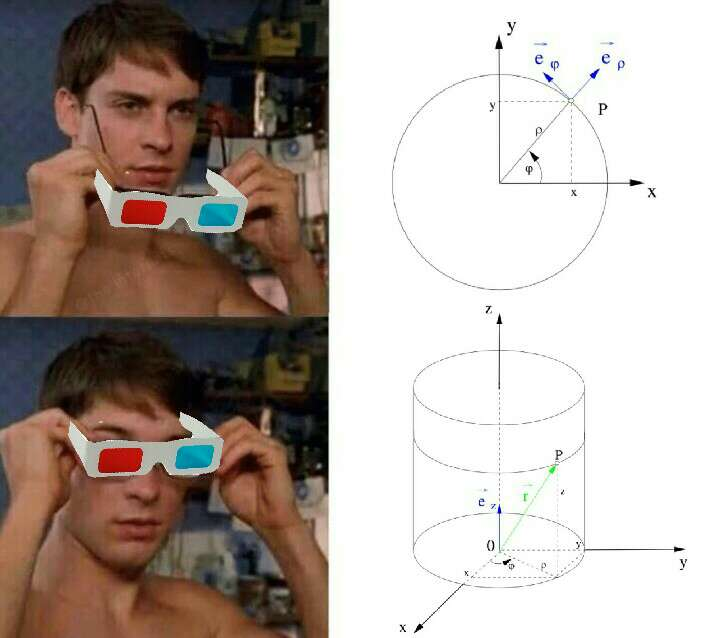
\includegraphics[width=.55\textwidth]{Dateien/3D_Analysis.jpg}\\
    Analysis, aber diesmal in 3D!\\
\end{figure}
\vfill
Grüßt euch, dies sind die Community MfP3-Notizen. \\

Sissi und ich erstellen sie als Nachbereitung der Vorlesung und sie dienen als eine schnelle Quelle von Definitionen und einfachen Beispielen (um sich einen Überblick zu verschaffen), wichtigen Bemerkungen aus den Übungen, sowohl als Klausurnotizen. Wir bewundern die informellen Notizen zum MfP1- und MfP2-Tutorium von Robin Löwenberg und Fabian Balzer und haben uns entschloßen mit dem gleichen Stil weiterzumachen, da es keine MfP3 und MfP4 Tutoriumnotizen mehr gibt. Die Templates wurden von Fabian erstellt und sind auf seiner Github-Seite verfügbar:  \url{https://github.com/Fabian-Balzer/MfP2-Notizen}. Zusätzlich benutzen wir das Lehrwerk Mathematik von Tilo Arens als eine Quelle von guten Beispielen. Das Buch können wir jedem empfehlen, der auch Giancoli mag und am besten an Beispielen lernt. Bei Anmerkungen oder Fragen schreibt uns einfach auf Whatsapp, Discord oder GitHub an. \\ 

Möge die Macht der endlosen zerbrochenen Kreiden mit euch sein :)

\cfoot{\pagemark}



\ifnum\value{reduce_to_selection}=0 {
    \tableofcontents
}\fi


%%%%%%%%%%%%%%%%%%%%%%%%%%%%%%%%%%%%%%%%%%%%%%%%%%%%%%%%%%%%%%%%%
\newpage
\section[Wiederholung]{Riemann-Integrale und Untermannigfaltigkeiten}
\subsection{Riemann-Integrale}\label{ssec:Riemann-Integrale}
\begin{Def}
{Ober- und Unterintegral}
Sei $f:[a,b]\rightarrow \R$ eine beschränkte Funktion. Das \red{Oberintegral} von $f$ ist die Zahl
$$\int_a^{*b}f(x)dx=\inf \{ \int_a^b \varphi(x)dx | \varphi \text{ Treppenfunktion mit } \varphi\geq f \} $$
Das \red{Unterintegral} von $f$ ist die Zahl
$$\int_{*a}^{b}f(x)dx=\sup \{ \int_a^b \varphi(x)dx | \varphi \text{ Treppenfunktion mit } \varphi\leq f \} $$
\end{Def}

\begin{Def}
{Riemann-integrierbare Funktion}
Eine beschränkte Funktion $f:[a,b]\rightarrow \R$ heißt \red{Riemann-integrierbar}, wenn $$\int_a^{*b}f(x)dx=\int_{*a}^bf(x)dx$$
\end{Def}
Ebenso ist es in der Analysis nützlich den Begriff des uneigentlichen Integrals zu verstehen, wenn der Definitionsbereich unbeschränkt ist.
\begin{Def}
{Uneigentliches Integral}
Sei $f:(a,b]\rightarrow \R$ nicht unbedingt beschränkt, aber für jedes Teilinterval $[\alpha, b] \in (a,b]$ integrierbar. Falls dann der Grenzwert
$$\lim_{\epsilon\rightarrow a}\int_\epsilon^{b} f(x)dx$$ existiert, so nennen wir $f$ über das Intervall $(a,b]$ \red{uneigentlich integrierbar}.
\end{Def}
\begin{Beispiel}
{Uneigentliches Integral}
Betrachten wir $\int_0^1 \frac{1}{\sqrt{x}}dx$. Dieses Integral kann als uneigentliches integral sinnvoll definiert werden:
$$\lim_{\epsilon\rightarrow 0}\int_\epsilon^1 \frac{1}{\sqrt{x}} dx =\lim_{\epsilon\rightarrow 0} [2\sqrt{x}]_\epsilon^1=\lim_{\epsilon\rightarrow 0}2\sqrt{1}-2\sqrt{\epsilon}=2$$
\end{Beispiel}
Die Gamma-Funktion $\Gamma(s)=\int_0^\infty t^{s-1}e^{-t}dt$ ist sehr nützlich, denn es gilt $\Gamma(s+1)=s\Gamma(s)$, also ist die Funktion perfekt dazu geeignet, um die Fakultät zu berechnen: $\Gamma(n)=(n-1)!$. Zusätzlich gilt $\Gamma(\frac{1}{2})=\sqrt{\pi}$.

\subsection{Topologie und Untermannigfaltigkeiten}\label{ssec:Topologie}
Gewisse topologische Begriffe sind auch im MfP3 sehr wichtig.
\begin{Def}
{Offene Kugel}
Die Teilmenge $\boxed{B_r(\xvec):=\Menge{\yvec\in X}{d(\xvec,\yvec)<r}\subseteq X}$ eines metrischen Raumes $(X,d)$ mit Abstandsfunktion $d$ heißt \red{offene Kugel} mit Mittelpunkt $\xvec$ und Radius $r$.
\end{Def}
\begin{Def}
{Inneres}
Für eine Teilmenge $A\subseteq X$ nennen wir die Vereinigung aller offenen Teilmengen das \red{Innere $\mathring{A}$} von $A$, also $\mathring{A}=\bigcup_{B\subseteq A}B$.
\end{Def}

\begin{Def}
{Abschluss}
Für eine Teilmenge $A\subseteq X$ nennen wir den Durchschnitt aller abgeschlossenen Mengen, die $A$ enthalten, den \red{Abschluss $\Bar{A}$} von $A$, also $\Bar{A}=\bigcap_{B\supset A, B\tx{ abgeschl.}}B$.
\end{Def}
\begin{Def}
{Rand}
Die Differenz aus diesen beiden Mengen ist dann der \red{Rand $\partial A$} von $A$, also $\partial A=\Bar{A}\setminus \mathring{A}$.
\end{Def}
\begin{Def}
{Kompaktheit}
Falls wir zu \underline{jeder} offenen Überdeckung $(U_i)_{i\in I}$ von $A\subseteq X$ eine endliche Teilüberdeckung, d.h. eine Einschränkung der Indexmenge $I$ auf eine endliche Menge $J\subseteq I$ finden, sodass $(U_i)_{i\in J}$ immer noch eine offene Überdeckung von $A$ ist, so nennen wir $A\subseteq X$ \red{kompakt}.
\end{Def}
\begin{Satz}
{Folgerung}{Kompakte Teilmengen sind abgeschlossen und beschränkt}
Jede kompakte Teilmenge $A\subseteq X$ eines metr. Raumes ist \underline{abgeschlossen}, \underline{vollständig} und \underline{beschränkt}.
\end{Satz}
\begin{Def}{Separable Räume und Dichtigkeit}
    Die Metrik $(X,d)$ heißt separabel, falls es eine abzählbare dichte Teilmenge in $X$ gibt. \\
    Eine Teilmenge $Y\subseteq X$ heißt dicht in $X$, wenn $\overline{Y}=X$.
    $$\forall \epsilon>0 \forall x\in X \exists y\in Y: d(x,y) <\epsilon$$
\end{Def}
Jetzt gehen wir über zu Untermannigfaltigkeiten und schließen die Wiederholung mit allgemeinen Mannigfaltigkeiten ab.
\begin{Def}
{Immersion}
Ist $\rg(f)=m\,\forall \pvec\in U$, d. h. die Abbildung hat den konstanten Rang der Dimension des \underline{Urbildraums}, so sagen wir, dass $f$ eine \red{Immersion} ist.\\
Das Differential $df:U\to\mathbb{R}^n$ ist dann injektiv. 
\end{Def}
Die $C^k(I,\R)$ ist eine $k$-fach stetig differenzierbare Funktion.
\begin{Def}
{$C^k$-Diffeomorphismen}
$C^k$-Abbildungen $f:U\to V$, die bijektiv sind und deren Umkehrabbildungen auch $C^k$ sind, nennen wir \red{$C^k$-Diffeomorphismen}.
\end{Def}
\begin{Beispiel}
{Bekannter Diffeomorphismus}
Die Abbildung $f:\mathbb{R}\to\mathbb{R}_+\setminus\MengeDirekt{0},\,f(x)=e^x$ ist mit $f^{-1}:\mathbb{R}_+\setminus\MengeDirekt{0}\to\mathbb{R},\,f^{-1}(x)=\ln(x)$ ein Diffeomorphismus, denn beide sind stetig differenzierbar, bijektiv und\\
$(f\circ f^{-1}=\Id_{\mathbb{R}_+\setminus\MengeDirekt{0}})\land (f^{-1}\circ f=\Id_\mathbb{R}).\,\checkmark$
\end{Beispiel}
Eine wichtige Eigenschaft von Diffeomorphisem ist, dass sie homoömorph sind.
\begin{Def}
{Untermannigfaltigkeit}
Wir nennen eine Teilmenge $M\subseteq\mathbb{R}^n$ eine \red{$m$-dimensionale Untermannigfaltigkeit}, falls für jeden der Punkte $\pvec\in M$ die folgenden Eigenschaften erfüllt sind:
\begin{itemize}
    \item Es gibt eine offene Umgebung $V\subseteq\mathbb{R}^m$ von $\pvec$.
    \item Es gibt eine $C^k$-Immersion\footnote{also eine Abbildung von Rang $m$} $F:U\to\mathbb{R}^n$, die eine offene Teilmenge $U\subseteq\mathbb{R}^m$ homöomorph auf $V\cap M$ abbildet.
\end{itemize}
\end{Def}
\begin{Def}
{Flächen und Hyperflächen}
Zweidimensionale Untermannigfaltigkeiten des $\mathbb{R}^n$ nennen wir \red{Flächen}.\\
$(n-1)$-dimensionale Untermannigfaltigkeiten des $\mathbb{R}^n$ nennen wir \red{Hyperflächen}.
\end{Def}
\begin{Satz}
{Satz}{Untermannigfaltigkeiten als Urbilder unter Abbildungen von konstantem Rang}
Sei $U\subseteq\mathbb{R}^n$ offen und $f:U\to\mathbb{R}^m$.
\begin{itemize}
    \item Ist $f$ eine $C^k$-Abbildung,
    \item hat $f$ konstanten Rang $r$ und
    \item ist $\qvec\in f(U)$,
\end{itemize}
so ist das Urbild\footnote{also alle Punkte, die auf $\qvec$ abgebildet werden} des Punktes $\qvec$ eine $C^k$-Untermannigfaltigkeit des $\mathbb{R}^n$ der Dimension \red{m=n-r}, also
\begin{equation}
    M:=f^{-1}(\qvec)\subseteq U.
\end{equation}
\end{Satz}
\begin{Beispiel}
    {Ein Beispiel von einer Untermannigfaltigkeit}
    Gegeben sind die beiden Funktionen
    \begin{equation*}
        f_1(x)=x_1^2+x_1x_2-x_2-x_3 \qquad f_2(x)=x_1^2+3x_1x_2-2x_2-3x_3
    \end{equation*}
    und die Menge
    \begin{equation*}
        C:=\Menge{x\in\mathbb{R}^3}{f_1(x)=f_2(x)=0}.
    \end{equation*}
    Wir behaupten nun, dass $C$ eine eindimensionale $C^{\infty}$-Untermannigfaltigkeit des $\mathbb{R}^3$ ist. Dazu betrachten wir die Funktion $f:\mathbb{R}^3\rightarrow\mathbb{R}^2$, gegeben durch
    \begin{equation*}
        f(x)=\Matrix{f_1(x) \\ f_2(x)}
    \end{equation*}
    und stellen fest:
    \begin{itemize}
        \item $f$ ist $\infty$-oft differenzierbar
        \item Das Differential ist
        \begin{align*}
            \text{d}f&=\Matrix{2x_1+x_2 & x_1-1 & -1 \\ 4x_1+3x_2 & 3x_1-2 & -3} \overset{Gauß}{\longrightarrow} \Matrix{2x_1 & x_1-1 & -1 \\ -2x_1 & -1 & 0} \\
            &\Rightarrow \text{rg}(f)=\text{rg}(\text{d}f)=2 \quad \forall x\in\mathbb{R}^3
        \end{align*}
        also ist $f$ eine Abbildung von konstantem Rang..
    \end{itemize}
    Die Behauptung folgt dann wieder direkt aus dem Satz über Untermannigfaltigkeiten als Urbilder unter Abbildungen von konstantem Rang. Die Untermannigfaltigkeit hat demnach auch die behauptete Dimension $3-2=1$.
\end{Beispiel}

Und nun zum krönenden Abschluss die allgemeinen Mannigfaltigkeiten.
\begin{Def}
    {Allgemeine Mannigfaltigkeiten}
    Gegeben seien ein metrischer Raum $M$, eine offene Überdeckung $(v_i)_{i\in I}$ von $M$ mit offenen Mengen $U_i \subseteq \mathbb{R}^m$ und Homöomorphismen 
    \begin{equation*}
        F_i:\, U_i\overset{\sim}{\rightarrow} V_i.
    \end{equation*}
    Man spricht dann von einer (abstrakten) m-dimensionalen $C^k$-Mannigfaltigkeit, wenn für je zwei offene Mengen $V_1,V_2\subseteq M$ mit Abbildungen $F_1$ und $F_2$ die Abbildung
    \begin{equation*}
        F_2^{-1}\circ F_1:\, F_1^{-1}(V_1\cap V_2) \rightarrow F_2^{-1}(V_1\cap V_2)
    \end{equation*}
    ein $C^k$-Diffeomorphismus ist.
\end{Def}
\newpage
\section[Fourier Reihen]{Fourier Reihen}
Die Fourier-Reihe ist ein wichtiges Instrument in der Physik, das uns ermöglicht (quasi-)periodische Funktionen mit einer Summe von vielen $\sin(x)$ und $\cos(x)$ zu approximieren.
\subsection{Fourier-Reihe}\label{ssec:Fourier}


\begin{Def}{Fourier-Koeffizient}
Sei $f:\R \rightarrow \C$ eine $2\pi$-periodische Funktion. Die komplexe Zahl
$$c_k=\frac{1}{2\pi}\int_0^{2\pi}f(x)e^{-ikx}dx$$
heißt das k-te \red{Fourier-Koeffizient}.
\end{Def}
\begin{Def}{Fourier-Reihe}
Die Reihe $$F(f)=\sum_{k=-\infty}^\infty c_ke^{-ikx}$$ heißt die \red{Fourier-Reihe} von $f$
\end{Def}
\begin{Beispiel}{Beispiel einer Fourier-Reihe}
Gegeben sei die Funktion $$f(x)=\begin{cases}1 & \mbox{wenn $0< x\leq \pi$}\\
0 & \mbox{wenn $\pi< x\leq 2\pi$}
\end{cases}$$
Wir wollen nun die Fourier-Reihe zu der $2\pi$-periodischen $f$ bestimmen, um die Funktion zu approximieren. Wir berechnen zuerst $c_0$.
$$c_0=\frac{1}{2\pi}\int_0^\pi 1 e^{0} dx + \frac{1}{2\pi}\int_\pi^{2\pi} 0 e^{0} dx = \frac{1}{2\pi}\pi - 0 = \frac{1}{2}$$
Nun berechnen wir $c_1$, um ein Gefühl zu entwickeln.
$$c_1=\frac{1}{2\pi}\int_0^\pi 1 e^{-ix}dx + \frac{1}{2\pi}\int_0^\pi 0 e^{-ix}dx = \frac{1}{2\pi}\int_0^\pi  e^{-ix}dx = $$
$$=\frac{1}{2\pi} \int_0^\pi \cos(x) - i\sin(x) dx =\frac{1}{2\pi}([\sin(x)]^\pi_0+i[\cos(x)]^\pi_0)=\frac{1}{2\pi}(0-2i)=-\frac{i}{\pi}$$
Anschließend berechnen wir $c_k$.
$$c_k=\frac{1}{2\pi}\int_0^\pi 1 e^{-ikx}dx + \frac{1}{2\pi}\int_0^\pi 0 e^{-ikx}dx=\frac{1}{2\pi}\int_0^\pi 1 e^{-ikx}dx=$$
$$=\frac{1}{2\pi} [\frac{ie^{-ikx}}{k}]_0^{\pi}=\frac{1}{2\pi} [\frac{i(\cos(kx)-i\sin(kx))}{k}]_0^\pi=\begin{cases}-\frac{i}{\pi k} & \mbox{k ungerade}\\ 0 & \mbox{k gerade}\end{cases}$$
Die Fourier-Reihe der Funktion $f$ ist dann
$$F(f)=\frac{1}{2}-\frac{i}{\pi}e^{-ix}+\frac{i}{\pi}e^{ix}-\frac{i}{3\pi}e^{-3ix}+\frac{i}{3\pi}e^{3ix}-\frac{i}{5\pi}e^{-5ix}+\frac{i}{5\pi}e^{5ix}\dots$$
Dies könnte man noch umschreiben:
$$F(f)=\frac{1}{2}+\frac{2}{\pi}\sin(x)+\frac{2}{3\pi}\sin(3x)+\frac{2}{5\pi}\sin(5x)+\dots$$
\begin{center}
    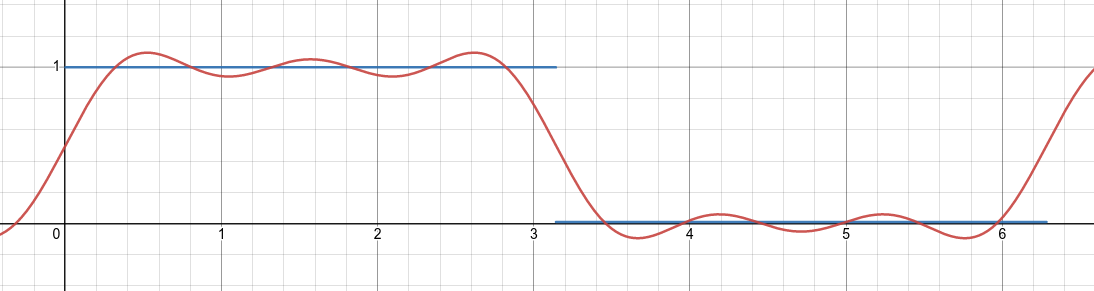
\includegraphics[width=.8\textwidth]{Dateien/Fourier_Beispiel.png}
\end{center}
Wie auf dem Bild zu sehen, approximieren wir mit jeden neuen Term die Funktion stückweise besser.

\end{Beispiel}
\begin{Satz}{Bemerkung}{Wichtige Fourier-Integrale}
Die folgenden Integrale sind sehr wichtig bei der Berechnung von Fourier-Reihen:
\begin{enumerate}
    \item $\int_0^{2\pi} \cos(kx)\sin(lx)dx=0, \mbox{ für $\forall k,l$}$
    \item $\int_0^{2\pi}\cos(kx)\cos(lx)dx=0 \mbox{ für $k\neq l$}$
    \item $\int_0^{2\pi}\sin(kx)\sin(lx)dx=0 \mbox{ für $k\neq l$}$
    \item $\int_0^{2\pi}\sin^2(kx)dx=\pi \mbox{ für $k\geq 1$}$
    \item $\int_0^{2\pi}\cos^2(kx)dx=\pi \mbox{ für $k\geq 1$}$
\end{enumerate}
\red{Wichtig!} Diese Beziehungen gelten nur für $k,l\in\N$.
\end{Satz}
\begin{Satz}{Bemerkung}{Fourier für un- und gerade Funktionen}
Es gilt $$F_n(f)=\frac{a_0}{2}+\sum_{k=1}^n (a_k\cos(kx)+b_k\sin(kx))$$
wobei $$a_k= c_k+c_{-k}=\frac{1}{\pi}\int_0^{2\pi}f(x)\cos(kx)dx$$
$$b_k=i(c_k-{c-k})=\frac{1}{\pi}\int_0^{2\pi}f(x)\sin(kx)dx$$
Wenn $f$ reellwertig ist, dann ist $c_{-k}=\overline{c_k}$ und $F_n(f)$ auch reellwertig. \\ \\
Ist $f$ gerade (d.h. $f(-x)=f(x)$), dann gilt
$$F_n(f)=\frac{a_0}{2}+\sum_{k=1}^n a_k\cos{(kx)}$$
Ist $f$ ungerade (d.h. $f(-x)=-f(x)$), dann gilt
$$F_n(f)=\sum_{k=1}^n b_k\sin{(kx)}$$
\end{Satz}
Eine weitere Anwendung der Fourier-Reihe ist auch das Beweisen von Folgen
\begin{Beispiel}{Folgenbeweise mit Fourier}
Wir sollen die Formel $\frac{\pi^2}{6}=1+\frac{1}{4}+\frac{1}{9}+\dots$ beweisen indem wir die Fourier-Reihe der $2\pi$-periodischen Funktion $f(x)=x^2$ im Intervall $-\pi\leq x\leq \pi$ bestimmen.
$$c_0=\frac{1}{2\pi}\int_{-\pi}^{\pi}x^2e^0dx=\frac{1}{2\pi}[\frac{x^3}{3}]_{-\pi}^{\pi}=\frac{1}{2\pi}(\frac{\pi^3}{3}+\frac{\pi^3}{3})=\frac{\pi^2}{3}$$
$$c_k=\frac{1}{2\pi}\int_{-\pi}^{\pi}x^2e^{-ikx}dx=\frac{1}{k^2}$$
$$c_k=\begin{cases} \frac{1}{k^2} & \mbox{wenn $k$ gerade} \\
-\frac{1}{k^2} & \mbox{wenn $k$ ungerade}
\end{cases}$$
$$F_n(f)=\frac{\pi^2}{3}-2\cos(x)+\frac{1}{2}\pi\cos(2x)-\frac{2}{9}\cos(3x)+\dots$$
Nun setzen wir für $x$ den Wert $x=\pi$ ein und erhalten:
$$F_n(f(\pi))=\frac{\pi^2}{3}+2+\frac{1}{2}+\frac{2}{9}+\dots$$
Wir wissen, dass $f(\pi)=\pi^2$ und substrahieren $\frac{\pi^2}{3}$ von beiden Seiten
$$\frac{\pi^2}{3}=2+\frac{1}{2}+\frac{2}{9}+\dots$$
Nun teilen wir beide Seiten mit $2$ und erhalten
$$\frac{\pi^2}{6}=1+\frac{1}{4}+\frac{1}{9}+\dots$$
\end{Beispiel}




\subsection{Konvergenz der Fourier Reihe}\label{ssec:FourierKonv}
\begin{Def}
{2-Norm}
Sei $V$ der Vektorraum der $2\pi$-periodischen Funktionen $f:\R \rightarrow \C$, wobei $f$ Riemann-integrierbar ist. Dann ist die Hermitische Form 
$$||f||_2=\langle f,f\rangle = \frac{1}{2\pi}\int_0^{2\pi}f(x)\overline{f(x)}dx, \space f\in V$$
die \red{2-Norm} von $f$.
\end{Def}
\begin{Satz}{Satz}{Konvergenz der Fourier-Reihe im quadratischen Mittel}
Sei $V$ der Vektorraum der $2\pi$-periodische Funktionen $f:\R\rightarrow\C$, für die $f$ integrierbar ist. \\
i) Für $\forall f\in V$ gilt
$$||f||_2^2=\sum_{k=-\infty}^\infty |c_k|^2$$
ii) Die Fourier-Reihe von $f\in V$ konvergiert im quadratischen Mittel gegen $f$, d.h. $\lim_{n\rightarrow \infty}||f-F_n(f)||_2=0$.
\end{Satz}
Es gibt tatsächlich keine $2\pi$-periodische Funktion im $\mathcal{L}^2$, dessen Fourier-Reihe nicht fast überall konvergieren würde.


\end{document}